\section{Results: How Models Use the Window}
\label{sec:results-window}

As shown in Section~\ref{sec:results-gain}, history helps every model family; the families differ, however, in how long a window they can use. In this section, we compare tree ensembles and sequence models over windows of up to fifteen reports on the controlled grid and in the $25\times25$ runs, test whether the order of the reports matters, and compare the learned models with a classical tracking filter.

% src: docs/results_of_record/history_extended/ne_mixed/history_extended_summary.csv (XGB BASE 3.577 (h=3) -> 3.465 (h=15); RF 2.785 (h=3) -> 3.350 (h=15); CNN 8.339 (h=0) -> 2.486; GRU 1.424 at h=15, three seeds; BASE_A GRU 1.300, XGB 2.817, RF 3.146); centre_mixed (GRU BASE_A h=15 0.599, XGB 0.99); ne_mixed_lstm (1.399 vs 1.424); technical_documentation_revised.md 6.2 (GRU below the best tree in all eight set x AoA rows); RMa LOS accuracy, GRU h=15 (history_extended centre/ne_rmalos) vs RF h=3 (comparison_sets.csv): centre 51.0 vs 55.3 % (MAE 2.19 vs 3.32 m), NE 47.9 vs 55.4 % (2.48 vs 2.92 m); with AoA centre 68.5 vs 69.0 % (1.01 vs 1.38 m), NE 51.5 vs 58.2 % (1.87 vs 2.20 m); CLAIM_EVIDENCE_MAP.md C3 caveat
\noindent\textbf{Long windows.} The tree ensembles take their gain at one to three steps and then stop, whereas a GRU keeps improving with every added step up to $h=15$, and a 1D-CNN does so in most settings~(Figure~\ref{fig:history-extended}). In the mixed setting with the BS beyond the corner and without AoA, XGBoost is flat from $h=3$ on and Random Forest is worse at fifteen steps than at three, while the GRU reaches \SI{1.42}{\meter} against $3.35$ and \SI{3.46}{\meter} for the two trees. The same ordering holds with AoA and in all four combinations of propagation setting and placement tested, so that the ranking of the families at long history is the reverse of their ranking at no history. The GRU's advantage lies in mean error: on the RMa LOS sets, Random Forest at three steps matches or exceeds the GRU's accuracy at fifteen, while its mean error remains higher. A long short-term memory~(LSTM) network of the same size performs the same as the GRU~($1.40$ against \SI{1.42}{\meter}), so the gain comes from the sequence, not from the recurrent cell.

\begin{figure}[h]
  \centering
  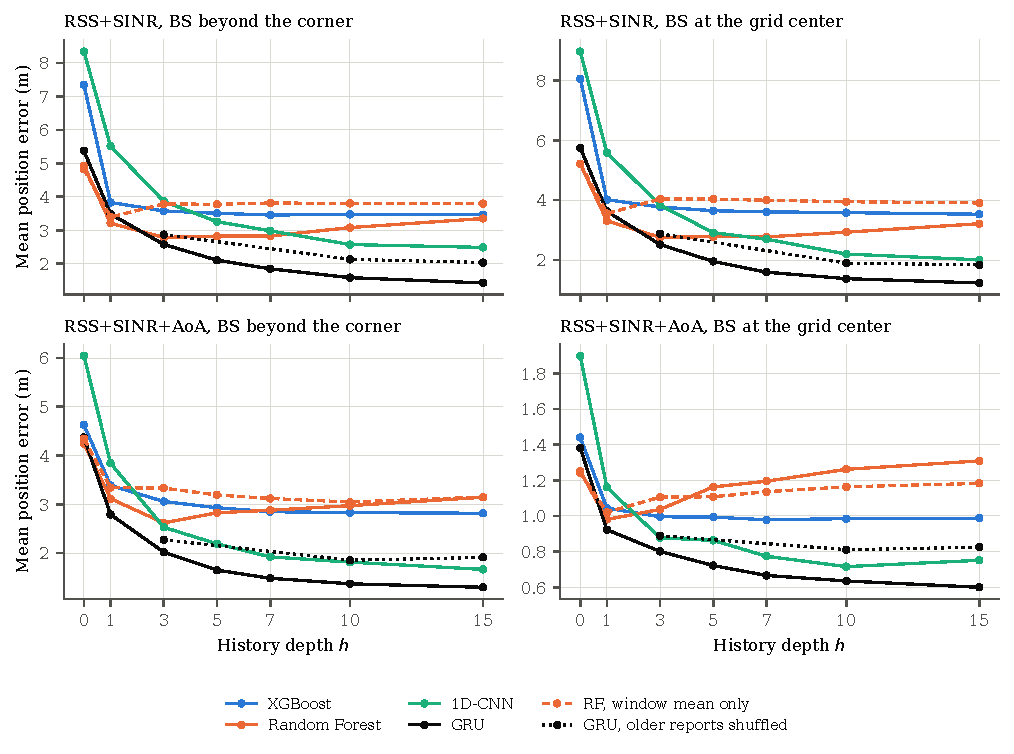
\includegraphics[width=0.95\textwidth]{fig_history_extended}
  \caption{Controlled grid, mixed propagation: mean position error against history depth $h$, without and with AoA, per BS placement. Trees and window-mean trees: single run; CNN and GRU: three seeds; shuffled GRU: two seeds.}
  \label{fig:history-extended}
\end{figure}
% src: figure_scripts/python/make_figures_followup.py history_extended_fig()

% src: docs/results_of_record/regression_25x25_2026_10/sequence_vs_trees/all_mae.md (GRU h=15 three seeds, spread <= 0.4 m; 1.3-5.0 m below the best tree at any depth; trees tuned at h=3; 400-epoch cap lowers the error by up to 0.9 m)
The $25\times25$ runs repeat the pattern at the macro-cell geometry. A two-layer GRU over the last $h+1$ reports keeps improving up to $h=15$ and has the lowest error in all six combinations of propagation setting and angle, $1.3$ to \SI{5.0}{\meter} below the best tree model at any depth~(Table~\ref{tab:cross-study}), while a 1D-CNN follows the same course slightly above it. History therefore lowers the error of the best model in this setting as well. The tree models use parameters tuned at $h=3$ and the GRU was still improving at its epoch limit, so the size of the gap is approximate.

% src: PLAN_AND_CHECKLIST.md 12.4 (window-mean trees; XGB h=5 4.52 vs 3.51 m); docs/results_of_record/history_extended/order_test_comparison.csv and technical_documentation_revised.md 6.2 table (older reports shuffled, current report kept, two seeds; GRU h=15 increase 19.0 % (RMa LOS NE, no AoA) to 49.0 % (mixed centre, no AoA, 1.235 -> 1.841 m); ne_mixed 1.424 -> 2.033 m; shuffled GRU below the best tree in 8/8 rows)
\noindent\textbf{The order of the reports.} Two controls show what the sequence models use. Giving the trees only the current report and the mean of the window does not make them keep improving; without AoA they are worse than the trees on raw lags from $h=3$ on. Permuting the older reports inside each window, in training and in test, while the current report keeps its place, raises the error of the GRU at $h=15$ by $19$ to \SI{49}{\percent} in all eight combinations of set, placement and angle, and the shuffled network gains little beyond ten steps while the ordered one keeps gaining. The shuffled GRU is nevertheless still more accurate than the best tree in all eight combinations, so only part of its advantage depends on order. We attribute this to the distance-ring ambiguity: a single RSS and SINR report is ambiguous between cells on the same signal contour around the BS, the mean of a window does not remove that ambiguity, and the ordered sequence of reports, which traces the movement across the contours, does. The history gain on the grid would then have two parts: an averaging part, shared by all models and the only part isolated in the macro cell~(Section~\ref{sec:results-mechanism}), and a sequence part that only recurrent and convolutional models exploit.

% src: results_of_record/tracking_filter/ne_mixed/tracking_filter.csv (RF snapshot 4.927 m; filter learned 0.714 m; generic 2 m kernel 0.93 m), technical_documentation_revised.md 6.2 l.261-278 (causal HMM forward filter; transition matrix learned from the training walks; caveats); history_irregular/ne_mixed{,_cnn}/history_irregular_summary.csv; paper/tables/T5_grid_baselines.md; CLAIM_EVIDENCE_MAP.md C8 (GRU keeps 80-90 % of its gain), C9
\noindent\textbf{A tracking filter and imperfect history.} History can also be used through a motion model instead of a learned window. A hidden Markov model~(HMM) forward filter on top of the Random Forest snapshot model combines the previous cell probabilities, propagated by a transition matrix, with those of the current report, and uses past reports only. With a transition matrix learned from the training walks, or with a generic kernel over distance, it lowers the error below that of the GRU~(Table~\ref{tab:grid-baselines}). The grid walk moves to a neighboring cell at every step and at constant speed, which a motion model suits well; the filter is therefore reported as a classical history-based baseline, and it was not run on the less regular trajectories of the macro cell. The learned models also tolerate imperfect history: when the older reports are missing at random or arrive at uneven gaps, and the models are trained with the same imperfection, the GRU keeps $80$ to \SI{90}{\percent} of its gain over the snapshot model and remains more accurate than XGBoost with complete history.

\begin{table}[h]
  \centering
  \caption{Controlled grid, mixed propagation, BS beyond the corner, RSS and SINR: mean position error~(m) with complete and imperfect history.}
  \label{tab:grid-baselines}
  \small
  \begin{tabular}{@{}llccc@{}}
    \toprule
    Model & Use of history & Complete & \SI{30}{\percent} missing & Uneven gaps \\
    \midrule
    Random Forest, current report only & none & $4.93$ & $4.90$ & $4.93$ \\
    XGBoost, $10$ older reports & learned window & $3.45$ & $4.07$ & $3.93$ \\
    1D-CNN, $10$ older reports & learned sequence & $2.49$ & $3.38$ & $3.01$ \\
    GRU, $10$ older reports & learned sequence & $1.59$ & $2.06$ & $1.99$ \\
    Random Forest + HMM, generic motion & motion model & $0.93$ & $1.16$ & $1.41$ \\
    Random Forest + HMM, learned motion & motion model & $0.71$ & $0.98$ & $1.27$ \\
    \bottomrule
  \end{tabular}
\end{table}
% src: paper/tables/T5_grid_baselines.md (uneven gaps: mean 2 steps; learned models trained with the same imperfection; CNN three seeds, GRU two, others single run)
